\documentclass[10pt]{beamer}

%%%
% PREAMBLE FOR THIS DOC 
%%%
%https://tex.stackexchange.com/questions/68821/is-it-possible-to-create-a-latex-preamble-header
\usepackage{/Users/miw267/Repos/latex_preamble/beamer_preamble}



%%% TRY TO RESHOW TOC AT EACH SECTION START (with current section highlighted)
% Reference: https://tex.stackexchange.com/questions/280436/how-to-highlight-a-specific-section-in-beamer-toc
\newcommand\tocforsect[2]{%
  \begingroup
  \edef\safesection{\thesection}
  \setcounter{section}{#1}
  \tableofcontents[#2,currentsection]
  \setcounter{section}{\safesection}
  \endgroup
}


%%%% HERES HOW TO DO IT CORRECTLY
% FIRST IN .STY FILE, DO
%\usetheme[sectionpage=none]{metropolis}
% THEN AT EACH SECTION DO
%\begin{frame}{Outline}
%  \tableofcontents[currentsection]	
%\end{frame}



%\setbeamertemplate{navigation symbols}{}
%\setbeamertemplate{footline}[frame number]{}


%%%
% DOCUMENT
%%%

\begin{document}

%\maketitle

%% Title page frame
%\begin{frame}
%    \titlepage 
%\end{frame}





\title{Friday 09/04/2026: Counterexample}
\author{CSCI 246: Discrete Structures}
\date{Textbook reference: Sec. 6, Scheinerman}

\begin{frame}
    \titlepage 
\end{frame}


\begin{frame}
\small 


\begin{myyellowbox}[title=Today's Agenda]
\begin{itemize}
	\item Weekly quiz (15 mins)
	\item Review previous group exercises ($\approx$ 15 mins)
	\item Mini-lecture ($\approx$ 5 mins)
	\item Group exercises ($\approx$ 15 mins)	
\end{itemize}
\end{myyellowbox}

%\vspace{-.2cm}

\begin{mygreenbox}[title=Quiz Set up]
\begin{itemize}
\item \textbf{Sheet of paper}: Please bring your own sheet of paper to class each day for quizzes if possible. However, if you don't have any, you are welcome to take a blank sheet of paper from the stack in the front of the room.
\item \textbf{Write your last name on the back}: Please write your first and last name on the front of the page where you will do your work.  Then, on the BACK of the page, please write your last name in large letters. This will help us return the graded quizzes efficiently.
\item \textbf{Rules of conduct}: For all quizzes in the course, you should use only paper and pencil.  Please close your computers and textbooks, and put away your cellphones.     
\end{itemize}
\end{mygreenbox}




\end{frame}






\begin{frame}

 \begin{myredbox}[title=Weekly Quiz \#1]  
\begin{enumerate}
	\item  \textit{(Sec. 3 -- Definition.)}  State whether each of the following is true or false; use Definition 3.2 to justify your answers: (a) $3 \mid 100$, (b) $-3 \mid 3$, (c) $0 \mid 4$, (d) $4 \mid 0$, (e) $0 \mid 0$.
	\item \textit{(Sec. 4 -- Theorem.)} Consider these two statements: (i) If A, then B, (ii) If (not B), then (not A).  Are these two statements identical, or not? Justify your answer through an argument using truth tables.
	\item \textit{(Sec. 4 -- Theorem.)}  Write out the truth table for the logical connective \textit{if and only if}. 
\end{enumerate}
\end{myredbox}

\vfill 
\begin{mygreenbox}[title=Reference Material: Scheinerman Definition 3.2] Let $a$ and $b$ be integers.  We say $a$ is \textit{divisible} by $b$, written $b \mid a$, provided there is an integer $c$ such that $bc=a$. 	
\end{mygreenbox}

\end{frame}



%\begin{frame}{Observation on Sec. 5 (Proofs) reading quiz}
%
%\begin{myyellowbox}[title=\textbf{Observation}] 
%A number of students wrote out expressions that look something like
%\[ 2|x + 2|y = 2|z\]
%\end{myyellowbox}
%
%\begin{myredbox}[title=\textbf{Warning}] 
%This expression has no meaning.    Note from the definition of divisibility (see below) that $2|x$ is itself \textit{already} an equation.  The notation $2|x$  \textit{means} that there is an integer $a$ such that $2a=x$.	
%\end{myredbox}
%
%
%\vfill 
%\begin{mydef}[title=Definition (\textbf{Divisible})]
%Let $a$ and $b$ be integers.  We say that $a$ is \textit{divisible} by $b$ (notated as $b|a$) provided there is an integer $c$ such that $bc=a$.  
%\end{mydef}
%
%\end{frame}


\begin{frame}[standout]
Question: How do you give a counterexample to \\
\qq{A implies B}? 	
\end{frame}


\begin{frame}{Unidirectional implication: Counterexample}
\colorbox{blue!30}{\textbf{Recall.}} Here's the truth table for unidirectional implication.
\begin{center}
\begin{tikzpicture}
\node[inner sep=0pt] (tbl) {%
\renewcommand{\arraystretch}{1.35}%
\begin{tabular}{cc|c}
\alert{A} & \alert{B} & $\overbrace{\alert{A} \implies \alert{B}}^{\text{If \alert{A}, then \alert{B}}}$ \\
\hline
T & T & \green{T} \\
T & F & \red{F} \\
F & T & \green{T}  \\
F & F & \green{T}  \\
\end{tabular}};
\only<2->{%
  \draw[black, line width=2pt] ([yshift=-0.23cm]tbl.center) ellipse (1.9cm and 0.32cm);
  \node[anchor=west, font=\Large] (lbl) at (2.65,-0.23) {counterexamples live here};
  \draw[black, line width=1.2pt, ->] (lbl.west) -- ++(-0.6,0);
}
\end{tikzpicture}
\end{center}

\vfill 
\only<3->{So we want to try to find a case where the antecedent (\alert{A})  holds, but the consequent (\alert{B}) is false.}
\only<4->{Let's try to apply this.}

\vfill 
\only<5>{\colorbox{blue!30}{\textbf{Proposition.}} If you live in Montana, then you live in Bozeman.}
\only<6->{\colorbox{blue!30}{\textbf{Proposition.}} If
  $\underbrace{\text{you live in Montana}}_{\alert{A}}$, then
  $\underbrace{\text{you live in Bozeman}}_{\alert{B}}$.}
\vfill 

\only<7->{\colorbox{blue!30}{\textbf{Counterexample.}}} \only<8->{Matt lives in Helena. So he lives in Montana (\alert{A} is true) but not in Bozeman (\alert{B} is False).}

\end{frame}

\begin{frame}[standout]
Question: How do you give a counterexample to \\
\qq{A if and only if B}? 	
\end{frame}



\begin{frame}{Bidirectional implication: Counterexample}
\colorbox{blue!30}{\textbf{Recall.}} Here's the truth table for bidirectional implication.
\begin{center}
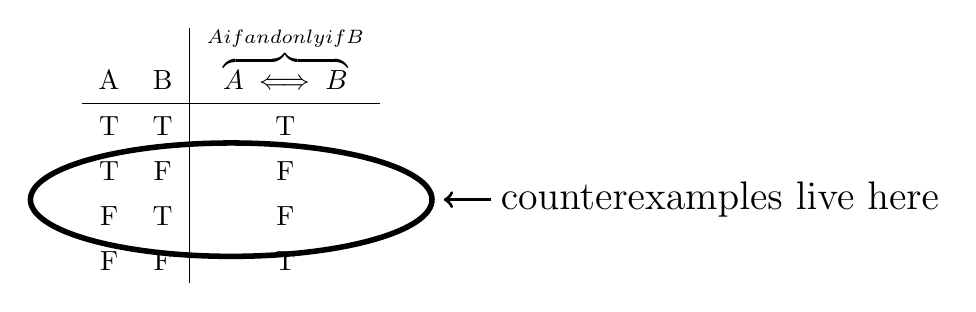
\begin{tikzpicture}
\node[inner sep=0pt] (tbl) {%
\renewcommand{\arraystretch}{1.35}%
\begin{tabular}{cc|c}
\alert{A} & \alert{B} & $\overbrace{\alert{A} \iff \alert{B}}^{\text{\alert{A} if and only if \alert{B}}}$ \\
\hline
T & T & \green{T} \\
T & F & \red{F} \\
F & T & \red{F}  \\
F & F & \green{T}  \\
\end{tabular}};
\only<2->{%
  \draw[black, line width=2pt] ([yshift=-0.56cm]tbl.center) ellipse (2.55cm and 0.72cm);
  \node[anchor=west, font=\Large] (lbl) at (3.3,-0.56) {counterexamples live here};
  \draw[black, line width=1.2pt, ->] (lbl.west) -- ++(-0.6,0);
}
\end{tikzpicture}
\end{center}

\vfill 
\only<3->{So we want to try to find a case where the truth values for \alert{A} and \alert{B} don't match. Let's try to apply this.}

\vfill 
\only<4>{\colorbox{blue!30}{\textbf{Proposition.}} A state is Montana if and only if it borders Canada.}   
\only<5->{\colorbox{blue!30}{\textbf{Proposition.}}   $\underbrace{\text{A state is Montana}}_{\alert{A}}$ if and only if 
  $\underbrace{\text{it borders Canada}}_{\alert{B}}$.}
\vfill 

\only<6->{\colorbox{blue!30}{\textbf{Counterexample.}} Michigan borders Canada (\alert{B} is true) but it is not Montana (\alert{A} is False).}

\end{frame}


\begin{frame}[standout]
Group Exercises \\
HINT: Unravel definitions!!
	
\end{frame}


\begin{frame}{Random group assignments}
\footnotesize
\begin{columns}
\begin{column}{0.33\textwidth}
Ashley, Isabelle: 4 \\ 
Bailey, Tanna: 1 \\ 
Blaisdell, Olyver: 5 \\ 
Brown, Ashton: 5 \\ 
Brown, Jonathan: 10 \\ 
Cardenas, Dominic: 12 \\ 
Cutler, George: 4 \\ 
Fabik, Roland: 3 \\ 
Fellows, Audrey: 7 \\ 
Fitzgerald, Ryan: 5 \\ 
Fuller, Ryan: 2 \\ 
Griffen, Clara: 9 \\ 
Grutsch, Tanner: 1 \\\end{column}
\begin{column}{0.33\textwidth}
Hager, Nathan: 3 \\ 
Horner, Jayden: 2 \\ 
Johnson, Jaret: 6 \\ 
Kintzel, Samantha: 12 \\ 
Lameres, Alexis: 11 \\ 
Lee, Holden: 9 \\ 
Mayala, Reece: 2 \\ 
McLean, Connor: 1 \\ 
Mcbride, Daniel: 8 \\ 
Miller, Maverick: 13 \\ 
Moss, Emily: 10 \\ 
Mousseau, Matthew: 6 \\ 
Neuman, Evan: 4 \\\end{column}
\begin{column}{0.33\textwidth}
Putnam, John: 7 \\ 
Ramos, Vydel: 13 \\ 
Rathbun, Jedidiah: 11 \\ 
Roberts, Matthew: 8 \\ 
Roller, Nathan: 13 \\ 
Ryan, Otis: 8 \\ 
Shevtsov, Timothy: 9 \\ 
Sinclair, Aidan: 11 \\ 
Smith, Charles: 7 \\ 
Stensland, Emma: 6 \\ 
Thiessen, Logan: 3 \\ 
Thompson, Jaiden: 12 \\ 
Vath, Ethan: 10 \\\end{column}
\end{columns}
\end{frame}


\begin{frame}{Group exercises}
\begin{enumerate}
	\item Disprove: If $a$ and $b$ are integers with $a|b$, then $a \leq b$.
	\item Disprove: If $p$ and $q$ are prime, then $p+q$ is composite.
	\item What does it mean for an if-and-only-if statement to be false? What properties should a counterexample for an if-and-only-if statement have?
	\item Disprove: An integer $x$ is positive if and only if $x+1$ is positive.
\end{enumerate}

%\vfill  \vfill 
%(Optional.) If you have extra time, you might try these for extra practice:
%\vspace{-0.5cm}
%\begin{enumerate}
%	\item[a.] Disprove: If $a$,$b$, and $c$ are positive integers with $a|bc$, then $a|b$ or $a|c$.
%	\item[b.] Disprove: If $p$ is prime, then $2^p-1$ is also prime.
%\end{enumerate}

\end{frame}



\begin{frame}{Group exercise \#1: Solution}

\textbf{Problem.} Disprove: If $a$ and $b$ are integers with $a|b$, then $a \leq b$.
\vfill 
\pause 
\textbf{Solution.} Let $a=5$ and $b=-5$. We will show that for this choice of $a$ and $b$, the hypothesis holds (i.e. $a|b$), but the conclusion doesn't (i.e. $a>b$).  By definition of divisibility, $a|b$ means that there is an integer $c$ such that $ac =b$. In this case, we need to show that there is an integer $c$ such that  $5c=-5$.  Indeed, the equation holds for $c=-1$.  Therefore, $b|a$, and the hypothesis holds.  However, clearly $a>b$, and so the conclusion fails. 
%\vfill 
%\textbf{Solution (shorter).} Let $a=5$ and $b=-5$. We will show that the hypothesis holds (i.e. $5|-5$), but the conclusion doesn't (i.e. $5>-5$).  To verify the hypothesis $5|-5$, note that there is an integer $c=-1$ such that  $5c=-5$.  We immediately see that $5>-5$, and so the conclusion fails.
%\vfill 
%\textbf{Remark.} In here and the following solutions , I provide longer solutions to clarify the logic for students who are struggling. However, in practice, feel free to provide shorter solutions, such as the one above.
\end{frame}


\begin{frame}{Group exercise \#2: Solution}

\textbf{Problem.} Disprove: If $p$ and $q$ are prime, then $p+q$ is composite. \pause 
% 
\vspace{-.1cm}
%
\begin{mygreenbox}[title=Reference: Scheinerman Def. 3.5]
An integer $s$ is called \textbf{prime} provided that $s>1$ and the only positive divisors of $s$ are $1$ and $s$. 
\end{mygreenbox}
 %  
\begin{mygreenbox}[title=Reference: Scheinerman Def. 3.6]
A positive integer $a$ is called \textbf{composite} provided that there is an integer $b$  such that $1<b<a$ and $b \mid a$. 
\end{mygreenbox}
%
\vspace{-.2cm}
%
\pause 
\textbf{Solution.}  Let $p=2$, $q=3$, and $r=p+q=5$.  We will show that for the counterexample, the hypothesis holds (i.e. $2$ and $3$ are prime), but the conclusion doesn't (i.e. $r=2 + 3 = 5$ is not composite). We know that $p=2$ is prime by the definition of prime below, since have that $2>1$ and its only positive divisors are $2$ and $1$.  A similar statement shows that $q$ is prime.  Hence, $p$ and $q$ are prime, and the hypothesis holds.  Moreover, $r=p+q$ is prime, and therefore not composite, and so the conclusion fails.


   
\end{frame}


\begin{frame}{Group exercise \#3: Solution}

\textbf{Problem.} What does it mean for an if-and-only-if statement to be false? What properties should a counterexample for an if-and-only-if statement have?
\vfill 

\textbf{Solution.} Recall from the group exercises of Sec. 4 (Theorems) that $A \iff B$ is identical to $(A \implies B) \, \texttt{and} \, (B \implies A)$.  Hence, we can show that $A \iff B$ fails by showing that either $A \implies B$ fails or $B \implies A$ fails.
\vfill 
\pause 
\textbf{Remark.} We will encounter this strategy again when we do a group exercise on DeMorgan's law in Sec. 7, Boolean Algebra.
\end{frame}

\begin{frame}{Group exercise \#4: Solution}

\textbf{Problem.} An integer $x$ is positive if and only if $x+1$ is positive.
\pause 
\vfill 
\textbf{Recall.} As discussed in group exercise \#3, we can show that $A \iff B$ fails by showing that $B \implies A$ fails OR by showing that $A \implies B$ fails. 
\vfill 
\pause 
\textbf{Solution.}  Let $A$ be the proposition that an integer $x$ is positive, and $B$ be the proposition that $x+1$ is positive.  We show that $A \iff B$ fails by showing that $B \implies A$ fails.   That is, we show that there exists a case where $B$ is true, but $A$ is false.  Take $x=0$. Then $B$ is true (since $x+1=1$ is positive), but $A$ is false (since $x=0$ is not positive).   
\end{frame}




\end{document}
